\documentclass[15pt,a4paper,oneside]{article}
\usepackage[T1]{fontenc}
\usepackage[utf8]{inputenc}
\usepackage[english]{babel}
\usepackage{fancyhdr}
\usepackage{graphicx}
\usepackage{listings}
\usepackage{color}
\usepackage{textcomp}
\usepackage{float}
\usepackage{tabularx}
%\usepackage{frontespizio}
\usepackage{multirow}
\usepackage{amsmath}
\usepackage{booktabs}
\usepackage{caption}
\usepackage{amssymb}
\usepackage{wrapfig}
\usepackage{subfig}
\usepackage{caption}
\usepackage{longtable}
\usepackage{hyperref}
\usepackage{multicol}
\usepackage{sidecap}
\hypersetup{%
    pdfborder = {0 0 0}
}
\usepackage{verbatim}
\lstset{basicstyle=\small\ttfamily,keywordstyle=\color{black}\bfseries,language=java,escapeinside={<@}{@>}}
\pagestyle{fancy}
\lhead{Fumagalli - Mariani - Mastellone}
\chead{}
\rhead{Tinfinity}
\lfoot{}
\cfoot{}
\rfoot{\thepage}
\renewcommand{\headrulewidth}{0.4pt}
\renewcommand{\footrulewidth}{0.4pt}
\sidecaptionvpos{figure}{c}

\begin{document}

\thispagestyle{empty}
\enlargethispage{60mm}
\begin{center}
\Large{\textsc{Politecnico di Milano}}\\
%\vspace{5mm}
\large{Scuola di Ingegneria Industriale e dell'Informazione}\\
%\vspace{5mm}
\large{Corso di laurea magistrale in Ingegneria Informatica}\\
\vspace{7mm}
\begin{figure}[h]
\begin{center}

\includegraphics[scale=0.15]{./images/logo-polimi}
\end{center}
\end{figure}
\vspace{2mm}

\begin{huge}
\begin{center}
Tinfinity
\end{center}
\end{huge}
\vspace{25mm}

\begin{LARGE}
\begin{center}
Design and Implementation of Mobile Applications
\end{center}
\vspace{2mm}
\end{LARGE}
\vspace{20mm}


\begin{flushleft}
\begin{tabular}{l l }

\end{tabular}
\end{flushleft}
\vspace{5mm}

\begin{flushleft}
\begin{tabular}{l l }
Professor : Luciano Baresi\\
\end{tabular}
\end{flushleft}

\begin{flushright}
\begin{tabular}{l l }
Fumagalli Alberto & Matr. 888888\\
Mariani Sebastiano & Matr. 817781\\
Mastellone Riccardo & Matr. 852341\\
\end{tabular}
\end{flushright}

\vspace{43mm}
{\large{\bf Academic Year 2015-2016}}
\end{center}

\newpage
\tableofcontents
\listoffigures
\newpage


 % !TEX root = ../report.tex
\section{Introduction}
This report will describe the \emph{Tinfinity} application, a proximity chat system for iOS platforms. The first part will introduce the application with a high level description and then the report will focuse on the technical aspects.

% !TEX root = ../report.tex

\section{High level application description}

\subsection{Description}
Tinfnity is a mobile application that implements a proximity chat system aiming to connect people in the same area. In order to access this application, the user must connect his Facebook account and share some of his informations like photos and date of birth. This step, simplifies the login process and mitigates the fake users problem delegating the issue to Facebook. Once the user has been successfully logged in the application, he can discover all the people that are using Tinfinity near to him using the map as shown in Figure 1. If the user finds someone interesting on the map, he can tap on the marker and send a friendship request as shown in Figure 2.

\begin{multicols}{2}
\begin{figure}[H]
\centering
\centering
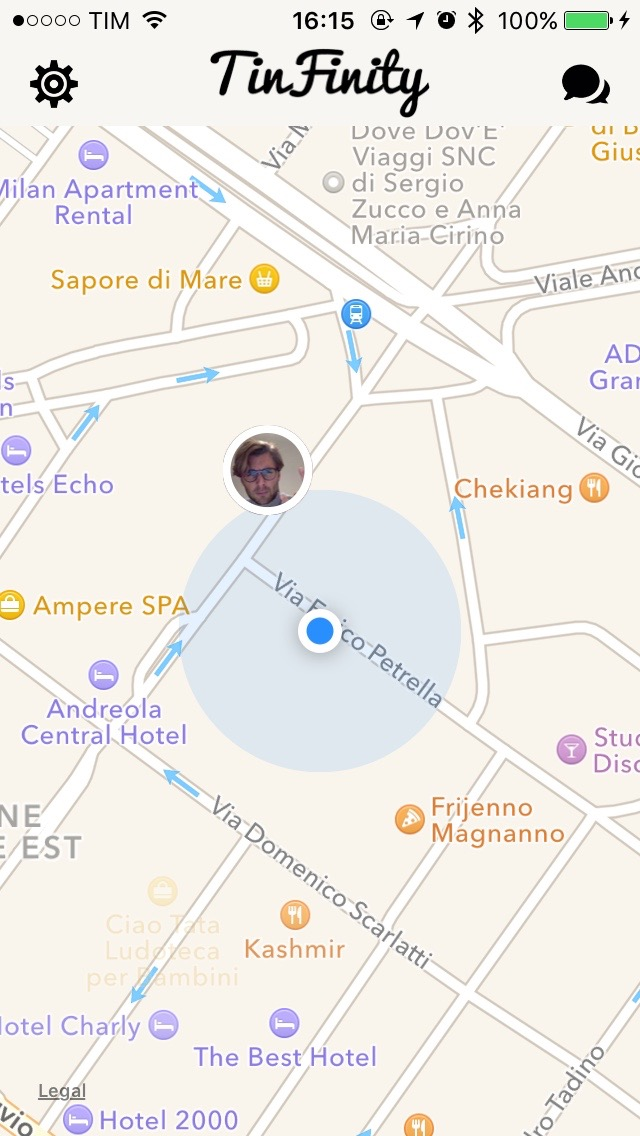
\includegraphics[scale=0.15]{./images/map.jpg}
\caption{\label{Users Map}Users Map}
\end{figure}

\begin{figure}[H]
\centering
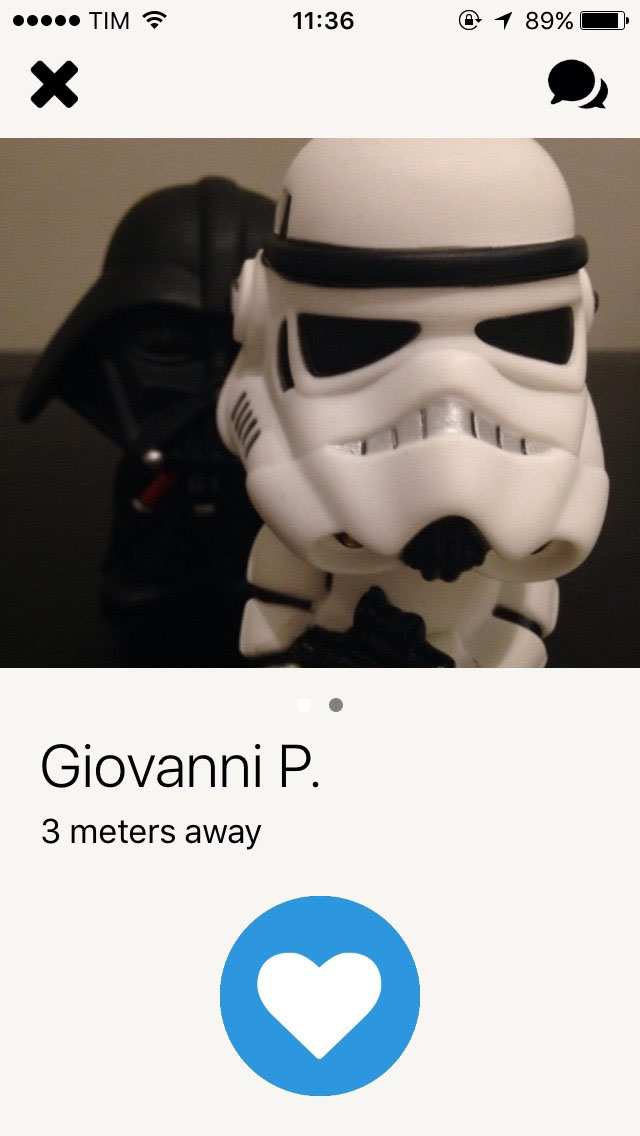
\includegraphics[scale=0.15]{./images/friendship_req.jpg}
\caption{\label{Friendship request}Friendship request}
\end{figure}
\end{multicols}

When and if recipient accepts the request, as shown in Figure 3, they can start chatting even when they are no longer close to each other, such a normal chat system as Whatsapp for example (shown in Figure 4), and maybe know each other directly in person. Additionaly the full name and the age of the other user are disclosed.

\newpage

\begin{multicols}{2}
\begin{figure}[H]
\centering
\centering
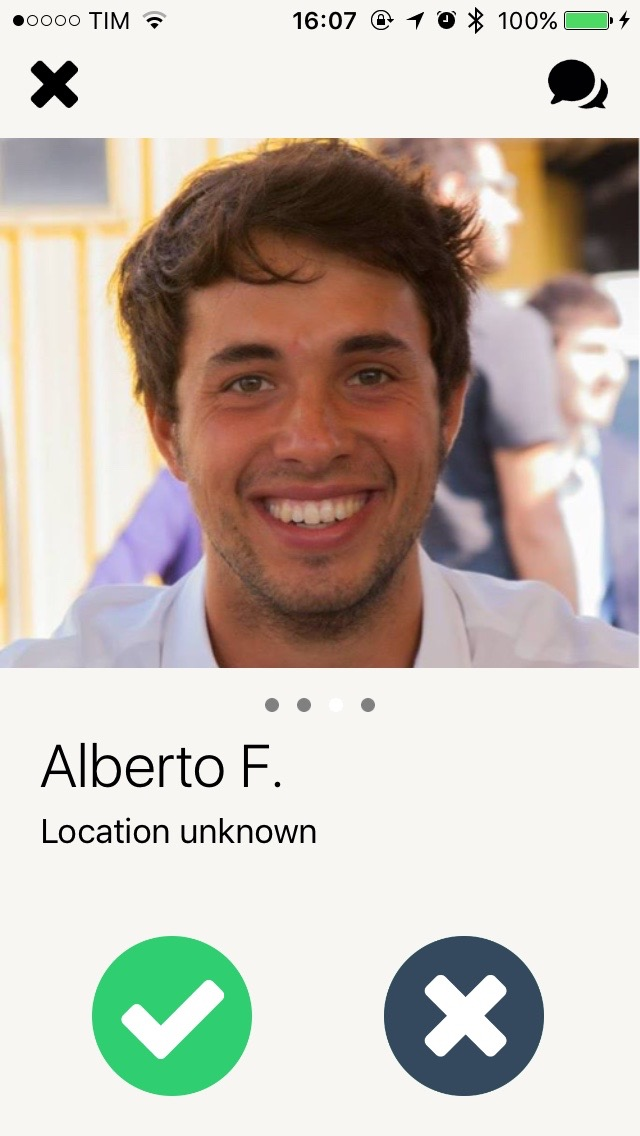
\includegraphics[scale=0.15]{./images/friendship_acc.jpg}
\caption{\label{Friendhip acceptance}Friendship acceptance}
\end{figure}

\begin{figure}[H]
\centering
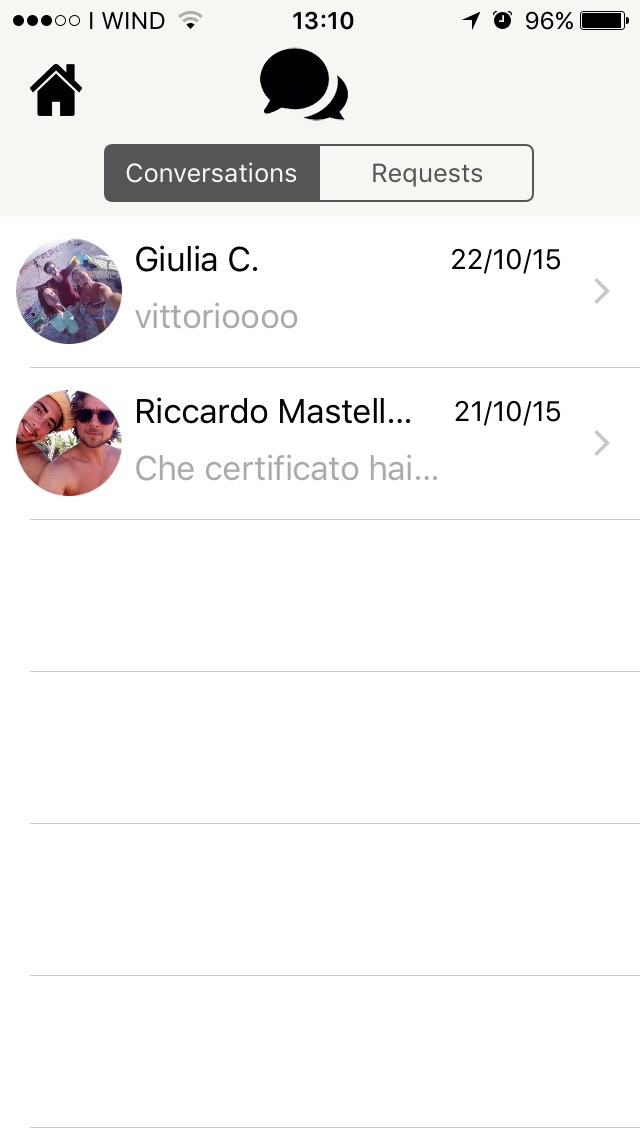
\includegraphics[scale=0.15]{./images/chat.jpg}
\caption{\label{Chat}Chat}
\end{figure}
\end{multicols}

The user can also see the informations relative to his profile (Figure 5) and personalise which photos have to be shared with other through the settings page as shown in Figure 6.

\begin{multicols}{2}
\begin{figure}[H]
\centering
\centering
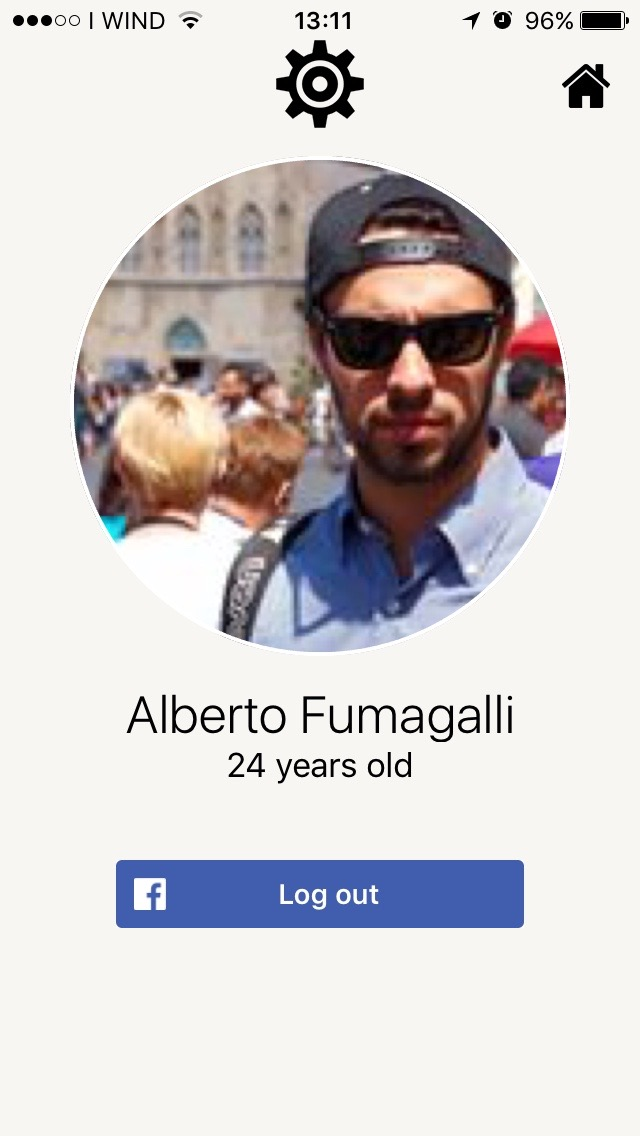
\includegraphics[scale=0.15]{./images/profile.jpg}
\caption{\label{Profile}Profile}
\end{figure}

\begin{figure}[H]
\centering
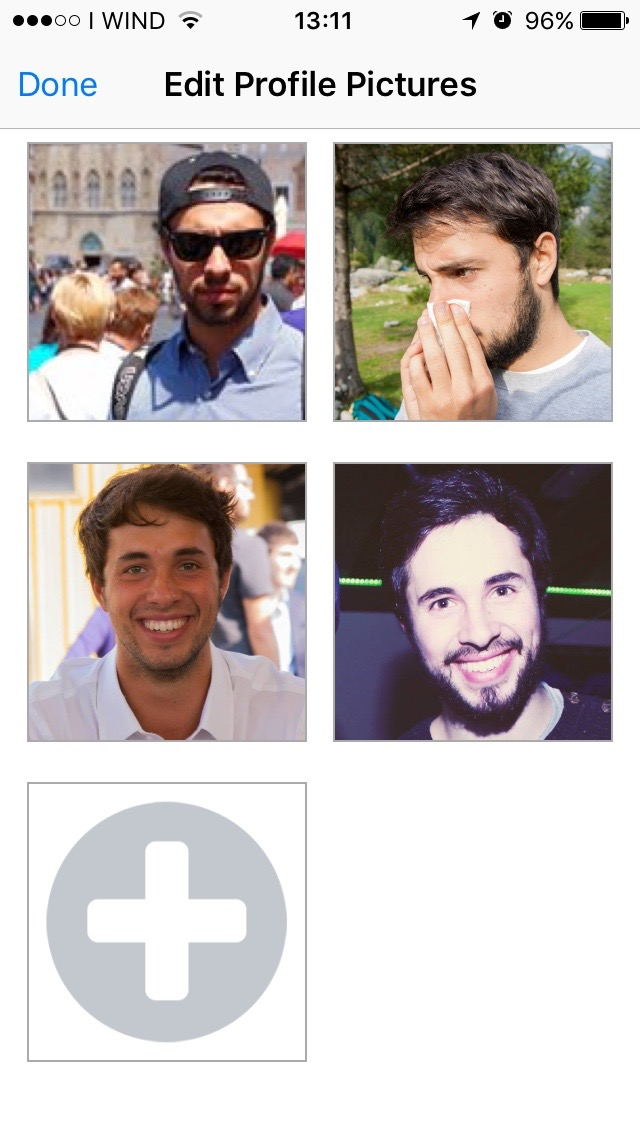
\includegraphics[scale=0.15]{./images/photo_selection.jpg}
\caption{\label{Profile}Profile}
\end{figure}
\end{multicols}

The application works in background and there is no need to open it in order to be localised by the others on the map.



\newpage
% !TEX root = ../report.tex
\section{Requirements}
In this section will be reported the functional and non functional requirements which have been identified in the analysis phase.
\subsection{Functional Requirements}
\begin{itemize}
\item Display to the user a map containing the position of other user within 800m from its position;
\item Provide a chat system and allow the user to interact with it;
\item Display the other users informations when request;
\item Enable the user to personalize the photos that have to be shared;
\item Enable the user to send a friendship requests and accept / decline the received one;
\item Create a web application in order to manage the chat system and the location system;
\item Create a push notification system in order to inform the user when a message is received;
\item Develop an iOS mobile version of the application;
\end{itemize} 


\subsection{Non Functional Requirements}
The non functional requirements are related to the devices which are target for the application:
\begin{itemize}
\item The application should run on devices with an iOS version > 8.4;
\end{itemize}
\newpage
 % !TEX root = ../report.tex
\section{Architecture}
The architectures of the application is composed by two main parts:
\begin{itemize}
\item A client iOS application
\item A server web application
\end{itemize}
The web application is necessary because it has to keep track of the users data, location and handle the chat system.

\newpage
 % !TEX root = ../report.tex
\section{Mobile application} 

\begin{figure}[H]
 \makebox[\textwidth][c]{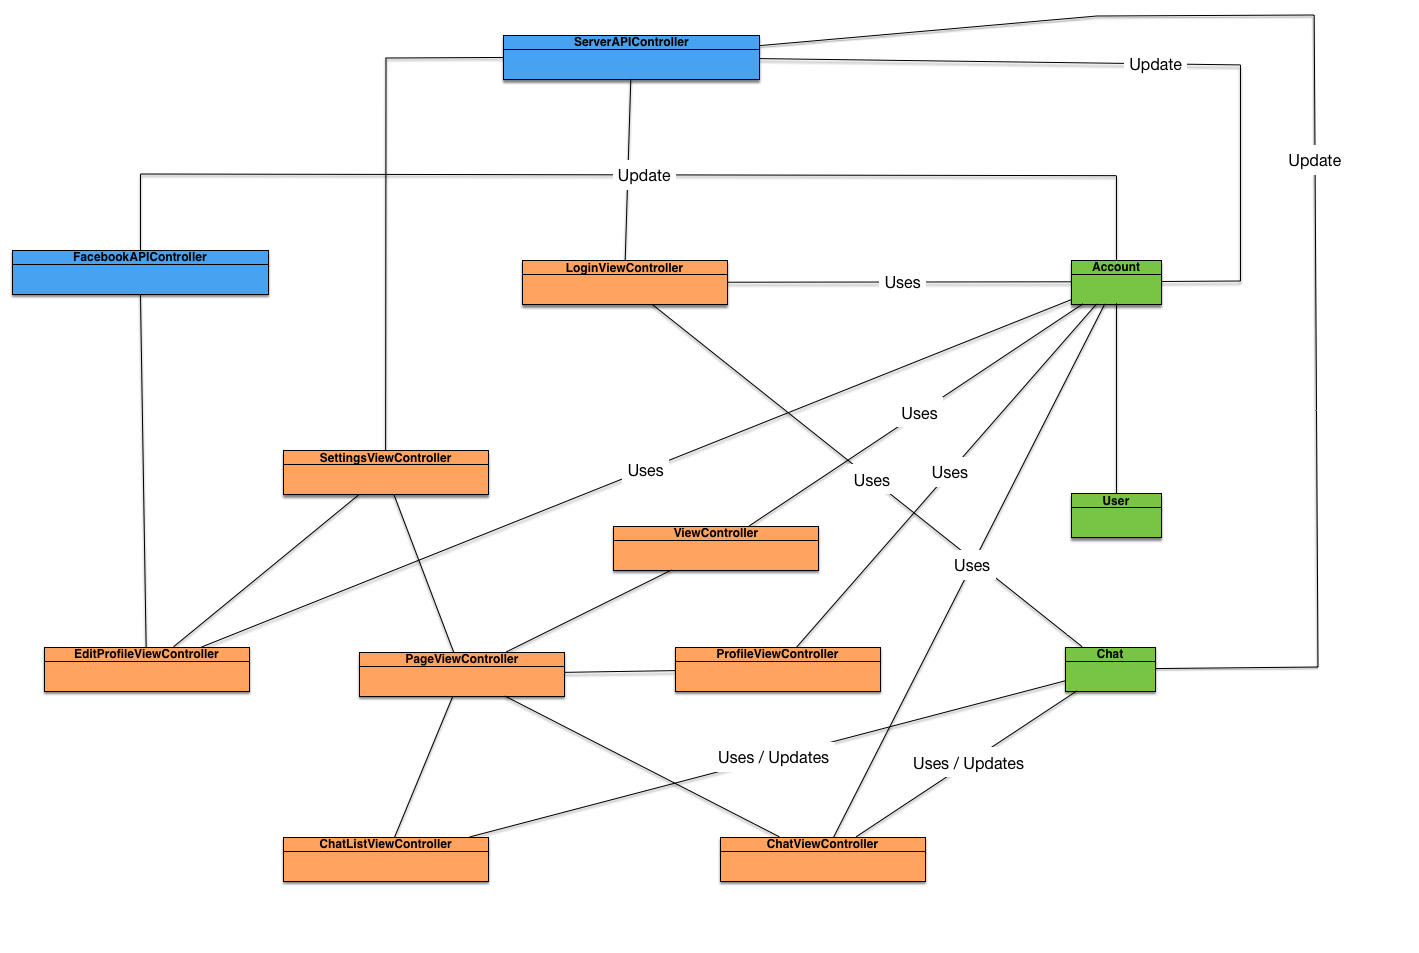
\includegraphics[width=1.6\textwidth]{./images/Tinfinity_general_class_diagram.png}}%
\caption{Simplified class diagram}
\end{figure}



The above class diagram shows a simplified version (only the most important classes are shown) of the application. The mobile application is based on eight main ViewController which handle the functionalities provided by Tinfinity:
\begin{itemize}
\item \textbf{LoginViewController} : Provides the login with Facebook functionalities and updates the account informations
\item \textbf{ViewController} : Provides to the user a map that shows where the other user are located and thei profiles.
\item \textbf{SettingViewController} : Provides a recap view of the informations about the user and the ability to change them.
\item \textbf{EditProfileViewController} : Provides the functionalities to decide which photos have to be displayed.
\item \textbf{ProfileViewController} : Provides a view that shows the profile of other users which have sent a friendship request, and the abilities to accept / decline it.
\item \textbf{ChatListViewController} : Provides a view with a list of the chat and the provides the functionalitiies to delete them.
\item \textbf{ChatViewController} : Provides a view with the conversation with the specified user and the abiluity to send messages.
\item \textbf{PageViewController} : Manages all the other views. It doesn't provide any functionality to the user, but it is used only for internal purposes.
\end{itemize}  

\subsection{LoginViewController} 
\begin{figure}[H]
 \makebox[\textwidth][c]{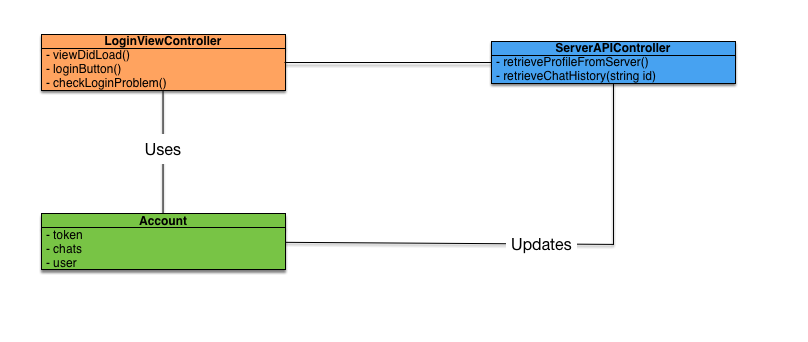
\includegraphics[width=1.6\textwidth]{./images/Tinfinity_LoginViewController.png}}%
\caption{LoginViewController class diagram}
\end{figure}

The LoginViewController manages the view that implement the login functionalities with Facebook and set up the initial settings relative to the account.

\begin{itemize}
\item \textbf{viewDidLoad()} : When the view is loaded this callback tries to check if there is already a valid Facebook OAuth token binded to the account. If the token is present and valid then the application will display the main view of the application.
\item \textbf{loginButton()} : This function is triggered when the login button is pressed. This function exploit the Facebook SDK in order to retrieve a valid Oauth token. If this operation succeed, then the other account settings, like the chat history, are retrieved and set and the main view of the application is displayed.
\end{itemize}


\subsection{ViewController} 
\begin{figure}[H]
 \makebox[\textwidth][c]{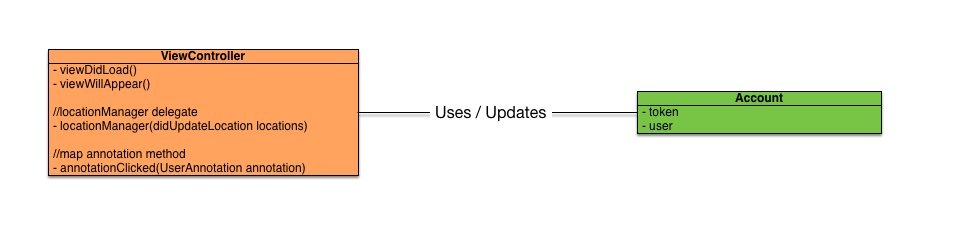
\includegraphics[width=1.6\textwidth]{./images/Tinfinity_ViewController.png}}%
\caption{ViewController class diagram}
\end{figure}


The ViewController manages the main view of the application and it show the map with the user location and the location of the other users around him. It is the delegate for the location manager and the mapView callback functions.

\begin{itemize}
\item \textbf{viewDidLoad()} : When the view is loaded this callback checks if the permissions needed in order to locate the user properly are given. if these are not given the map is hidden, otherwise the map is displayed and the user location is retrieved.
\item \textbf{viewWillAppear()} : Every time the view is shown the location of the user is updated.
\item \textbf{locationManager(didUpdateLocations error)} : Set the latitude and longitude of the user and add a marker on the map.
\item \textbf{annotationClicked(UserAnnotation annotation)} : When a marker of anopther is clicked the information relative to him are retrieved and passed to the ProfileViewController
\end{itemize}

\subsection{SettingsViewController} 
\begin{figure}[H]
 \makebox[\textwidth][c]{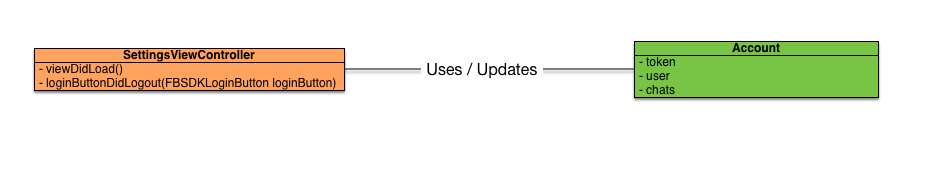
\includegraphics[width=1.6\textwidth]{./images/Tinfinity_SettingsViewController.png}}%
\caption{SettingsViewController class diagram}

\end{figure}

The SettingsViewController shows a view with the recap iof the user informations and implement the logout functionality.

\begin{itemize}
\item \textbf{viewDidLoad()} : When the view is loaded all the informations about the user, like the profile picture, are retrieved and displayed properly.
\item \textbf{loginButtonDidLogout()} : Exploit the Facebook SDK in order to invalidate the OAuth token and log out the user from the application.
\end{itemize}

\subsection{EditProfileViewController} 
\begin{figure}[H]
 \makebox[\textwidth][c]{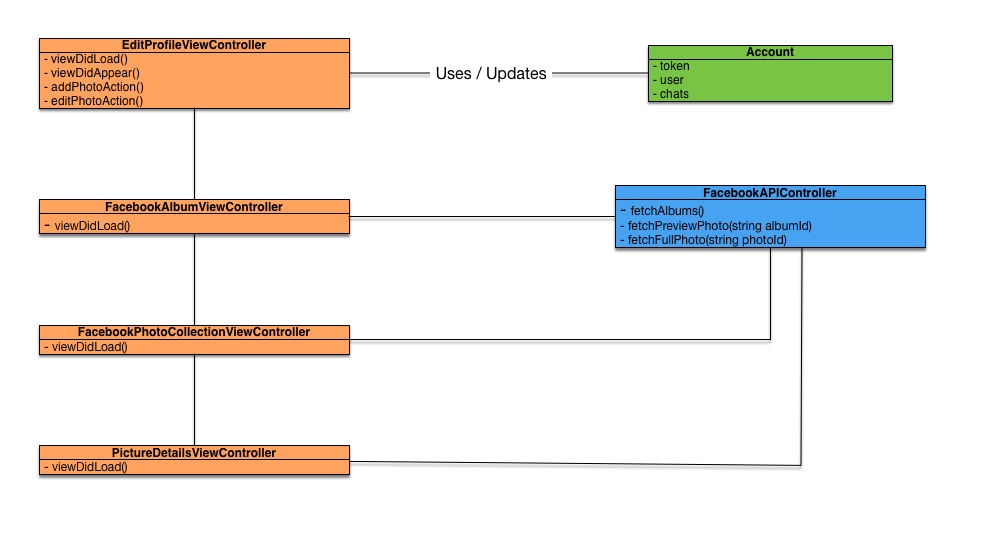
\includegraphics[width=1.6\textwidth]{./images/Tinfinity_EditProfileViewController.png}}%
\caption{EditProfileViewController class diagram}
\end{figure}


The EditProfileViewController and the other auxiliary ViewControllers (FacebookAlbumViewController, FacebookPhotoCollectionViewController and PictureDetailsViewController) provides the functionalities of the photo editing. The user here can decide which photos of his Facebook profile have to be displayed in the application.

\begin{itemize}
\item \textbf{viewDidLoad() (FacebookAlbumViewController)} : Fetches the Facebook photos album relative to the user.
\item \textbf{viewDidLoad() (FacebookPhotoCollectionViewController)} : Fetches the preview of the photos that are in the selected album.
\item \textbf{viewDidLoad() (PictureDetailsViewController)} : Fetches the high resolution version of the selected photo.
\end{itemize}


\subsection{ProfileViewController} 

\begin{figure}[H]
 \makebox[\textwidth][c]{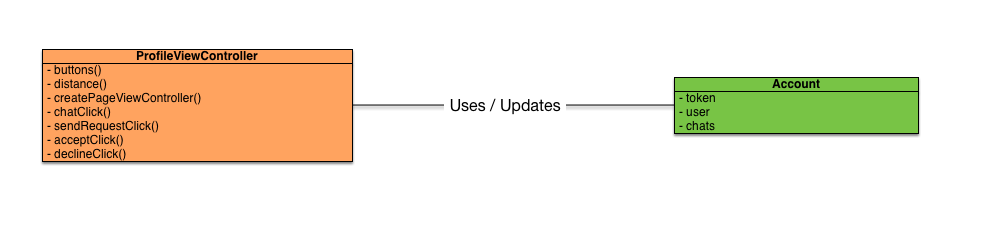
\includegraphics[width=1.6\textwidth]{./images/Tinfinity_ProfileViewController.png}}%
\caption{ProfileViewController class diagram}
\end{figure}


The ProfileViewController manages the view displyed when the user click on a marker on the map or when he receive a friendship request. this view shows all the details relative to the other user like the distance, his photos and his name and age. It provides also the functionalities in order to accept or decline a friendship request, send a new request, or start a new chat with the selected user.

\begin{itemize}
\item \textbf{buttons()} : Based on the reletionship with the other user, this function decides which buttons have to be displayed.
\item \textbf{distance()} : This functions calculate the distance between the user and the other selected user.
\item \textbf{createPageViewController()} : Creates the photos slideshows with the photos of the other user.
\item \textbf{chatClick()} : Start a new chat with the other user.
\item \textbf{sendRequestClick()} : Send a friendship request to the other user.
\item \textbf{acceptClick() / declineClick()} : accept / decline a received friendship request.
\end{itemize}


\subsection{Persistent Data Design}
\begin{figure}[H]
\centering
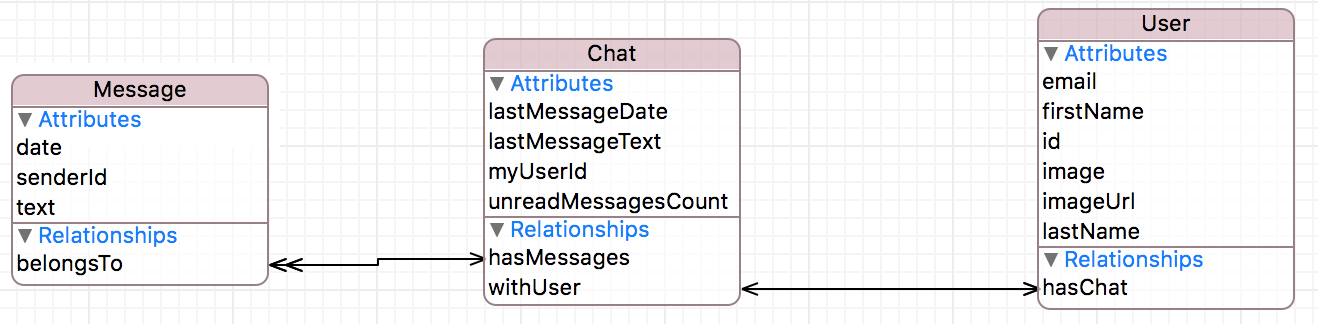
\includegraphics[width=1\textwidth]{./images/Tinfinity_CoreData.png}
\caption{Database}


The persistent Core Data is composed by 3 classes:

\begin{itemize}
\item \textbf{Message} : contains the informations of a single message(the date in which the message has been sent,the sender and the actual message text) and has a one-to-one relationship that associate it to a certain chat;
\item \textbf{Chat} : contains the information of a chat(the date and text of the last message that has been received, the id of the logged user and the counter of unread messages) and has two relationships, one is a one-to-many relationship with the message class, that associate the chat with all of his messages, and the other a one-to-one relationship with the User class, that represent the other user.
\item \textbf{User} : contains all the inforrmation of a user(email, firstname, lastname, id, the user image and its url) and has a one-to-one relationship with the chat that is associated with it.
\end{itemize}
\end{figure}








\newpage
% !TEX root = ../report.tex
\section{User Experience}

\subsection{Sender User Experience}

\begin{figure}[H]
 \makebox[\textwidth][c]{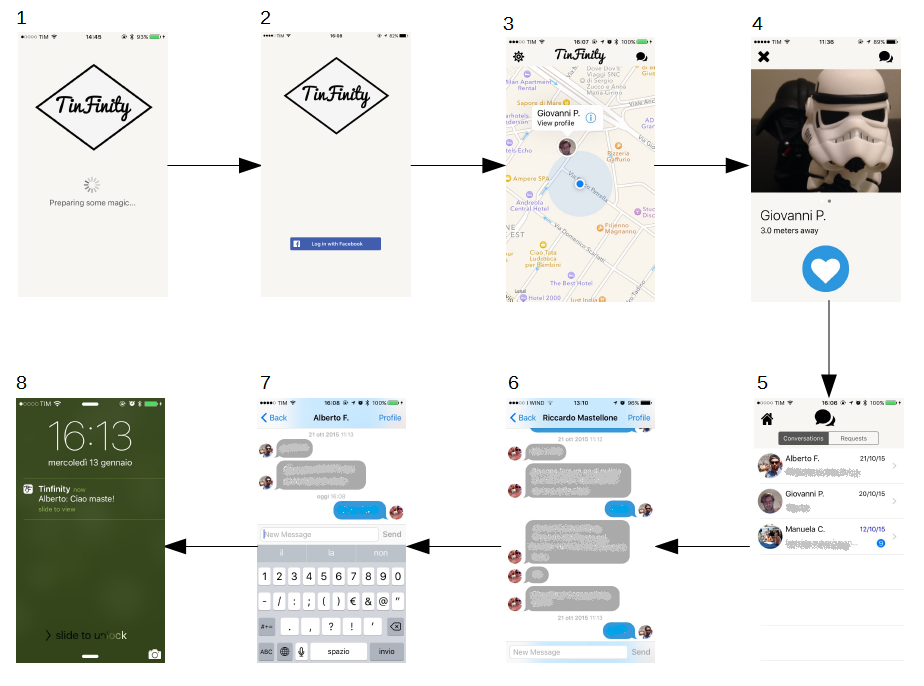
\includegraphics[width=1.6\textwidth]{./images/ux_sender.png}}%
\caption{Sender User Experience}
\end{figure}

\begin{enumerate}
\item The application launcher contacts the server in order to retrieve to check if there isa already a valid login token present

\item From the login view the user can inserts his Facebook username and password and log in to the application

\item From the main view the user can see the people around him and choose to look at an interesting profile

\item The user can send a friendship request

\item[5--8] When and if the other user accept the friendship request, they can start chatting as a normal chat application.
\end{enumerate}


\subsection{Receiver User Experience}

\begin{figure}[H]
 \makebox[\textwidth][c]{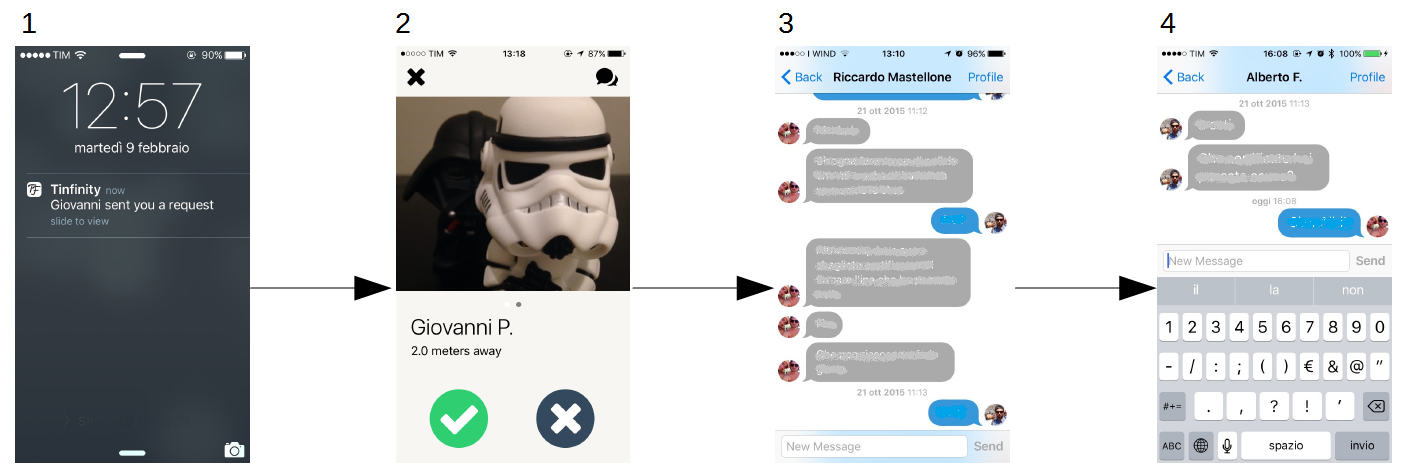
\includegraphics[width=1.6\textwidth]{./images/ux_receiver.png}}%
\caption{Receiver User Experience}
\end{figure}

\begin{enumerate}
\item The user receive a notification about a received friendship request 

\item The user can choose if the request has to be accepted or declined


\item[3--4] If the friendship is granted they can start chatting as a normal chat application.
\end{enumerate}

\newpage

\subsection{Photo selection User Experience}

\begin{figure}[H]
 \makebox[\textwidth][c]{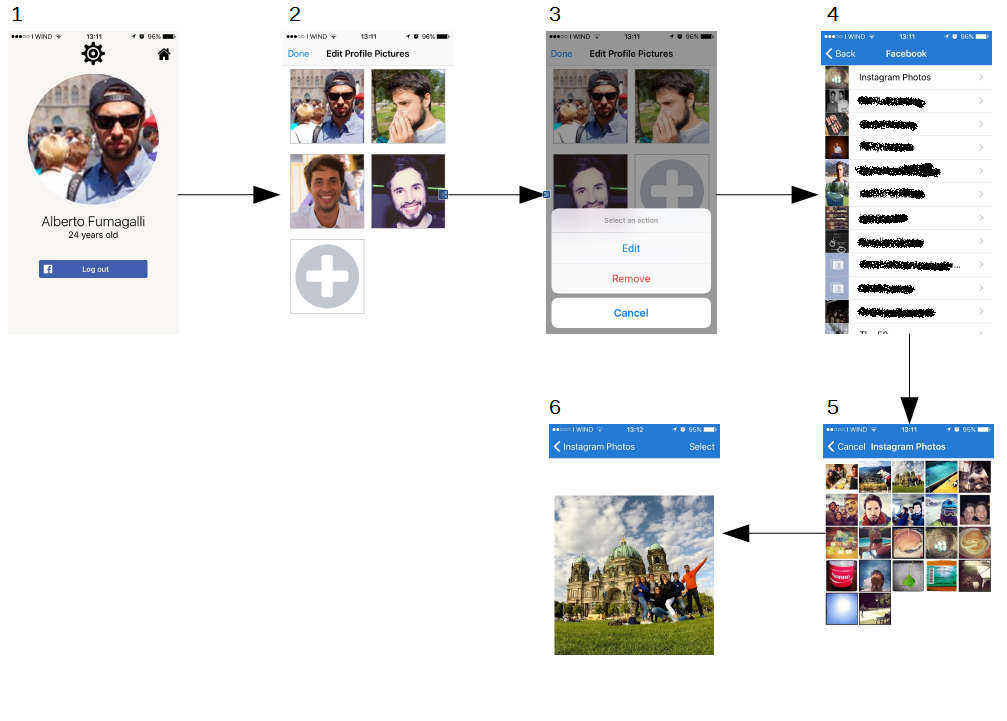
\includegraphics[width=1.6\textwidth]{./images/ux_photo_change.png}}%
\caption{Photo selection User Experience}
\end{figure}

\begin{enumerate}
\item From the settings view the user can tap on his photo profile in order to modify it or add other photos which will be visible by other users.

\item The user can tap on the '+' button and chose whether to add or change a current photo

\item All the photo albums of the Facebook account are displayed 

\item  All the photos of the selected album are displayed

\item  Finally tap on the select button the displayed photo is added to the user profile

\end{enumerate}
\newpage
 % !TEX root = ../report.tex
 
\section{Web app}
This web server has been developed to support the iOS Tinfinity application. 

It is written using Node.js with the Express framework and uses MongoDB as a database. These have been preferred over many alternatives for performance reasons, as they support a very high number of concurrent connections with very little resources. Additionally, websockets are natively supported using SocketIO, allowing a real-time, bidirectional and reliable chat system.

\begin{figure}[H]
 \makebox[\textwidth][c]{
\includegraphics[width=1.0\textwidth]{./images/schema_webapp.png}}%
\caption{Web app overview}
\end{figure}

The structure of the web server has been developed so to not be tightly coupled with the client architecture (iOS), hence other clients (e.g., Web, Android) can be easily created starting from the APIs documentation.

All the security checks are done server-side, not disclosing any unwanted information unless explicitly requested by the user.

MongoDB offers natively Geospatial data type support, and near users are retrieved directly querying the database with the user current position.

%\newpage
%\appendix
%% !TEX root = ../report.tex

\section{Work flow}
The workflow of our project can be divided in different phases, from the idea selection to the testing of the application. Our goal was to create something which would have made the experience at the EXPO both more interesting and educational. The growing technology related to the Augmented Reality were perfect for stimulating the visitors interest while the creation of the dishes from all over the world would have made the experience more challenging and instructive. The Augmented Reality feature is a core component in our application so the choice of the correct library was very important and the Metaio SDK has revealed to be a good decision because it provides all the functionality needed by us without having to buy the licence. Another important issue related to the Augmented Reality functionality was the creation of the 3D model representing the mascots. We aren't expert in 3D model creation, for this reason we tried to search already existing models and edit them in order to make them look more like nice mascots. The software which was very useful in this phase was Blender, an open source 3D graphics and animation software. Another important feature of our application is the creation of recipes by combining different ingredients; for this reason we needed to define in a precise way the set of ingredients, recipes and mascots we would insert in our application.
The most important phase from the development point of view was the structural analysis of the entire system. During this stage we have defined the classes organization of the Android application and we have discussed about the usefulness of a web application. At the end we come up with the idea that the web application not only can be used to provide dynamic content to the application but can also allow us to create and manage the database of receipts and ingredients. Using the documents redacted in the structural analysis phase we have implemented the web application based on the ExpressJS framework and using a MongoDB backend database. The data inside the web service are exported to a SQLite database in order to be used in the application. Finally the last two phases consist of implementing the Android application and testing in order to solve unexpected bugs.

% % !TEX root = ../report.tex
\section{Supports}


% % !TEX root = ../report.tex
\section{Testing}


\end{document}